\begin{appendix}
%=======================================================
\chapter{OMAP-L137 implementation}
Initially OMPA-L137 EVM was used to develop PMU. And considerable development was done but during a testing it got damaged and started malfunctioning. So, a brief description is given here about what all things were done and it's concept.

 OMAP-L137 EVM doesn't have Analog to Digital Converter on board hence an interfacing circuit is designed. While designing the ADC board following criteria were considered.
\begin{itemize}
	\item Good sampling rate: ~200 kSamples/Sec
	\item Minimum no of channels: 3 + 3 = 6 (3 - $\phi$ voltage and current) 
	\item Interfacing type: It should be memory addressable and voltage level compatible  to the EVM.
	\item Input type: FSS analog output is differential which can be configured as single ended and its voltage level is $\pm$10V
\end{itemize}
  
On basis of the above stated requirements several chips were filtered for the application and finally AD7864 was chosen. AD7864 is a high speed 4 channel simultaneous (dedicated) sampling successive approximation ADC with \textit{bi-polar input} having conversion time as low as $1.65 \mu s$. Chip's sampling rate can go as high as 500 ksps \cite{uguide:adc}. Chip's conversion sequence can be controlled through hardware as well as software, its default operating voltage of control and data pins is 5v but it has a special output voltage level shifter for interfacing it with 3.3v processors and controllers. A variant of the chip AD7864-1 was chosen as our ADC due to it's direct input voltage compatibility range of $\pm$ 10 V. This ADCs are fairly advance and hence they have been interfaced with a special asynchronous peripheral interfacing architecture called Extended Memory InterFace (EMIF-A), which is exclusively available in OMAP-L13x series processors.

 Extended Memory InterFace (EMIF) has two parts A \& B out of which EMIF-B is having \textit{Enhanced Direct Memory Access} controller (EDMA3) which enables the processor for multi-threaded rapid memory access and hence it is exclusively for highspeed SDRAM interfacing where as interface \textit{A} (EMIF-A) is developed for generic purposes, it's further details are given below:

\subsubsection{EMIF-A}
EMIF-A controller is a 16-bit databus based versatile controller \cite{uguide:emifa}, designed to interact with variety of devices like 
\begin{itemize}
	\item Single Data Rate (SDR) RAM
	\item Asynchronous devices like NAND \& NOR flash memory and SRAM
\end{itemize}

\begin{figure}[h]
	\centering
	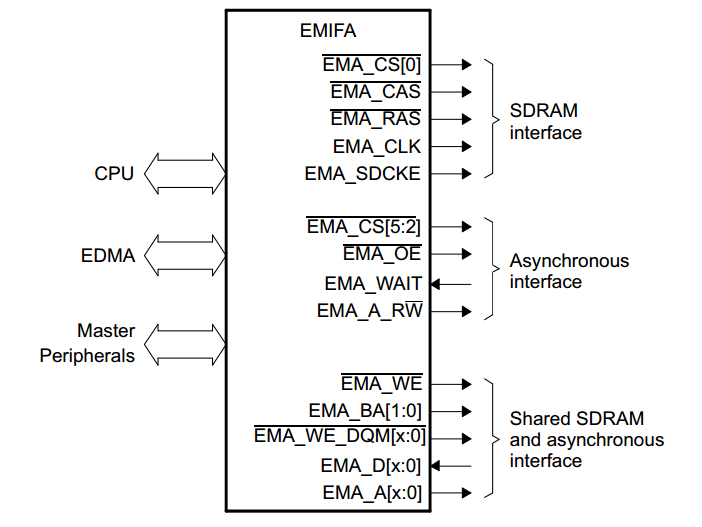
\includegraphics[scale=0.4]{fig/EMIFA.png}
	\caption{EMIFA Block Diagram \cite{uguide:emifa} }
	\label{fig:EMIFA}
\end{figure}

It contains lot of features to ease and facilitate the usage of asynchronous devices. A functional block diagram is given here in Fig: \ref{fig:EMIFA} It is apparent from Fig: \ref{fig:EMIFA}, that it has 4 chip selects and, read and write for them and 16 data channels. which makes it very convenient for interfacing multiple peripherals at a time. 


\begin{figure}[ht]
	\centering
	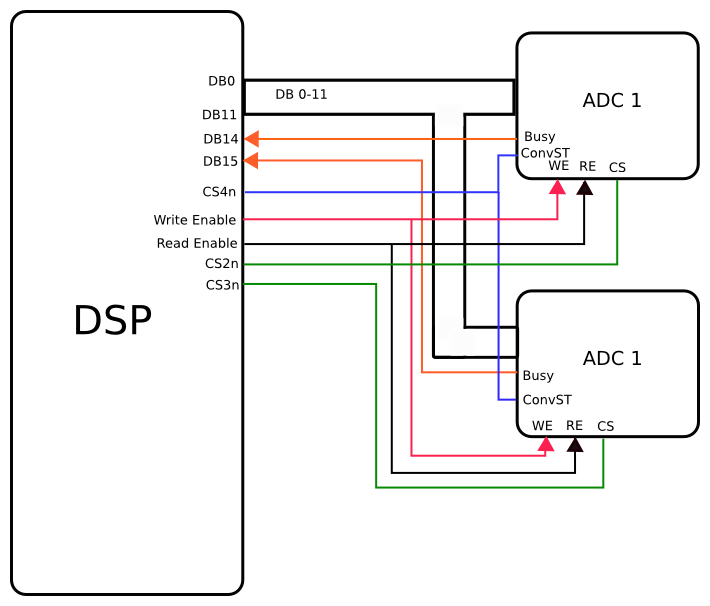
\includegraphics[scale=0.4]{fig/ADC_board.png}
	\caption{ADC Board block diagram}
	\label{fig:adc_board}
\end{figure}
Using the EMIF-A and the AD7864-1 a ADC board was designed for interfacing OMAP-L137 with Full Spectrum Simulator. Above Fig: \ref{fig:adc_board} shows the design logic of that ADC board. 


\subsubsection{ADC board Logic}
Due to EMIFA, interfacing of ADC board became quiet convenient rather than using pins in GPIO mode. So the logical flow of the board is as follows:

\begin{itemize}
	\item 6 input channels are required hence 2 ICs are used
	\item Chip Select (CS), Read, Write, and databits from 0 - 11 are directly available from the EMIFA interface, and they are shared with both the chips.
	\item AD7864 has sequence selection which has been configured through hardware, and Clock source has been kept internal. because of this both the pins \texttt{INT/EXT\_CLK} \& \texttt{H/S select}
	\item AD7864 has 3 control output \texttt{Busy}, \texttt{FIRSTDATA} and \texttt{EOC}. Out of these only \texttt{busy} is observed via a data line (data bits 16 \& 15). Data is \textbf{and}ed is not read until data line 15 \& 14 are not zero.
	\item AD7864 supports two kinds of data reading 1) Reading during the conversion 2)Reading after the conversion. Here we are going to use \textit{Reading After the conversion}, below is the timing diagram of the chip for understanding the proper functioning of the circuit.
\end{itemize}


\begin{figure}[h]
	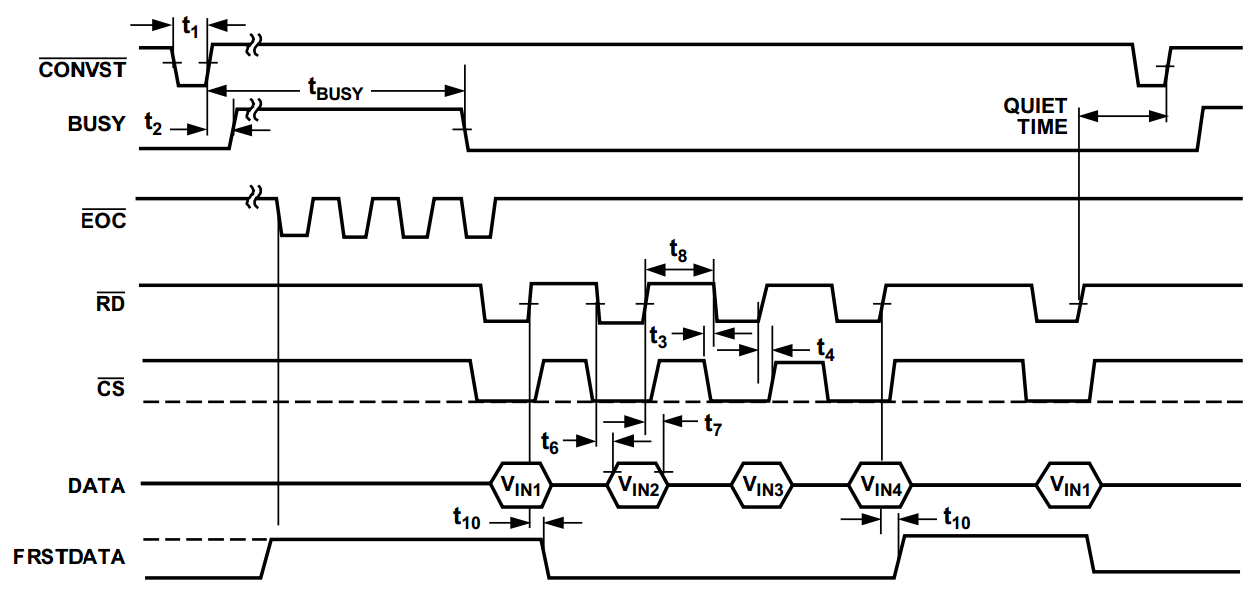
\includegraphics[width =\columnwidth]{fig/adc_time_diag.png}
	\caption{ADC Reading After the Conversion timing \cite{uguide:adc}}
	\label{fig:adc_timing}
\end{figure}
Now we will see the operation that takes place when sampling  is to be done:
\begin{itemize}
	\item Assert start of conversion (\texttt{CONVST}) is asserted via \texttt{EMA\_CS(4)}
	\item Due to this chip will start the conversion processes which will make \texttt{BUSY} high,
	\item Status of \texttt{BUSY}  will be checked via \texttt{DB15} \& \texttt{DB14} pins of the EMIFA header, for both the chips untill they are \texttt{low} again.
	\item The moment \texttt{BUSY} goes low, \texttt{EMA\_CS[2]} and \texttt{EMA\_A\_RE} are asserted with which AD7864 starts putting data on data lines. this processes of asserting is repeated for 4 times, for each channel. The same is done using \texttt{EMA\_CS[3]} for getting data from 2nd ADC chip.
\end{itemize}
Apart from ADC board another important component in PMU is GPS signal. A NavSynch CW-12TIM GPS receiver is will be interfaced. The receiver provides three type of output signal.
\begin{itemize}
	\item 1PPS - Synchronized with the start of the UTC second
	\item 10MHz FOUT - The maximum time interval error (MTIE) of this signal is 4us at the interval of 446.8 Ks.
	\item UART - Data communication port for UTC data and other control/status information
\end{itemize}
The receiver has an on board RTC which maintains the time information in loss of satellite fix.

\subsubsection{Software Implementation}
OMAP-L137 being a dual core asymmetric type processor it will run two instance of OSes or program, (i) DSP side and (ii) ARM side.  

\begin{itemize}
	\item \textbf{DSP Side:}
	DSP can be programmed in 2 ways (a) Boiler plate programming (b) Using an OS. Boiler plate programming would be the fastest running implementation yet a challenging task to accomplish, as all the necessary device drivers and interfacing has to be done manually. In case of OS based implementation, an abstraction layer is there which will have all the necessary device drivers already available, user just has to use the library and write a higher level C/C++ code. Though second approach seems lucrative, a compromise needs to be made in regards to the latency. Due to the existence of a kernel and a scheduler, the execution will be slow. In our device, our timing requirements were not very intensive and could have been met easily hence OS was use.
	
	Taxas Instruments, provides two OS options (a) DSP/BIOS (b) SYS/BIOS, DSP/BIOS being less flexible and slower as well as getting obsolete and phased out by TI, Sys/BIOS was chosen. Sys/BIOS provides preemptive multi-threading, hardware abstraction, real-time analysis, and configuration tools.The libraries are optimized for execution time and majority of them are written in assembly	language. The threading model provides threads for interrupts and tasks. Priorities and blocking characteristics of these can be easily controlled. For the application, all Sys/BIOS objects are configured statically and bound into a single image
	
	\item \textbf{ARM Side:} On the ARM side by default MontaVista OS was provided along with EVM. For our purpose, real-time micro kernel OS-- QNX RTOS was chosen. Officially QNX-6.4 is supported but QNX- 6.5 source can be modified to work on OMAP-L137. Few salient feature of QNX are 
	\begin{itemize}
		\item Micro kernel: Runs most of the functions as tasks which can be easily disabled reducing the size of memory footprint. The kernel is basically just a scheduler which allows smaller OS ticks to be handled efficiently. The PMU application requires features like the TCP/IP stack, I/O handlers, Timers and Memory Management. Rest of the overheads like filesystem, DMA, RTC, USB can be stripped off.
		\item TCP/IP stack: QNX has TCP/IP stack has all features and yet its tiny.
		\item  Multitasking: Two primary task run on ARM side, One of which sis to acquire \emph{time data word} from GPS, update the system time and to \emph{send data} packets over ethernet.
	\end{itemize}

\end{itemize}
It is very important to keep the memory footprint low as both the OSes use the same RAM and it has only 64 MB RAM, which is also being used for data storing.

\subsubsection{Implementation}
Strategy of implementation is as follows:
\begin{enumerate}
	\item Low level tasks of controlling ADC and sensing 1PPS will be done by DSP core.  Start of conversion, data ready and read will be asserted by DSP core. 
	\item Data received from the ADC upon which DFT computation will be performed and data will be passed to ARM via shared memory.
	\item ARM core running QNX will read the results from shared Memory and data packet will be formed which will be sent to the PDC.
	\item QNX will also communicate with GPS module to receive and decode time status word over UART. Time information will be used in time tagging the data before being sent over the network. 
\end{enumerate}
Before the board got damaged following things were implemented already implemented on it:
\begin{itemize}
	\item DSP core Timer was configured to assert start of conversion signal to ADC chip
	\item GPS 1 PPS signal was interfaced with one of the data pin EMIF-A, which was configured as GPIO, which was generating interrupt. 
	\item Testing of data read function was being carried out.
\end{itemize}

\chapter{Compiler Optimisation}

There are several compilation time and run time optimizations available with GCC suit which can really impact the performance of a program \cite{compilerOpti}. These options control various sorts of optimizations. Without any optimization option, the compiler's goal is to reduce the cost of compilation and to make debugging possible with the expected results. Turning on optimization flags makes the compiler attempt to improve the performance and/or code size at the expense of compilation time and possibly the ability to debug the program. There are 4 major levels of optimization defaults, that are provided by GCC. which are -O, -O1, -O2, -O3.
\begin{enumerate}
	\item \textbf{-O \& O1}
	Optimize. Optimizing compilation takes somewhat more time, and a lot more memory for a large function. With -O, the compiler tries to reduce code size and execution time, without performing any optimizations that take a great deal of compilation time.
	
	\item \textbf{-O2} Optimizes even more. GCC performs nearly all supported optimizations that do not involve a space-speed tradeoff. The compiler does not perform loop unrolling or function inlining when you specify -O2. As compared to -O, this option increases both compilation time and the performance of the generated code.
	
	\item \textbf{-O3} Optimize yet even more. -O3 turns on all optimizations specified by -O2 along with other flags listed in the table  
\end{enumerate}


Level \texttt{-O3} was used for optimizing the code for this project and \texttt{O3} is the highest level of optimization possible by GCC. The list of flags passed by O3 are listed below:


 



\begin{table}[h]
	\centering

	\caption{Compiler Optimization Flags}
	\label{my-label}
	\textit{
	\begin{tabular}{|l|l|}
		\hline
-ffast-math & -floop-optimize   \\ \hline
-fdefer-pop  & -foptimize-sibling-calls   \\ \hline
 -fdelayed-branch & -fguess-branch-probability \\ \hline 
-fthread-jumps & -fcse-follow-jumps  -fcse-skip-blocks   \\ \hline
-fmerge-constants & -frerun-cse-after-loop  -frerun-loop-opt  \\ \hline
-fstrength-reduce		& -fgcse   -fgcse-lm   -fgcse-sm \\ \hline
 -fdelete-null-pointer-checks 		&  -fcaller-saves\\ \hline
-fregmove 		& -fexpensive-optimizations \\ \hline
-fsched-interblock -fsched-spec	&  -fschedule-insns -fschedule-insns2 \\ \hline
-fstrict-aliasing &  -freorder-blocks  -freorder-functions \\ \hline
-fpeephole2		& -falign-functions  -falign-jumps \\ \hline
-falign-loops  -falign-labels		&  -fcrossjumping \\ \hline
-fif-conversion & -fif-conversion2 \\ \hline
 -fcprop-registers & -fforce-mem \\ \hline
	\end{tabular}
}
\end{table}

More detailed description of each flag can be found on this GCC C compiler \texttt{man} pages \cite{compilerOpti}.

It worthwhile to note here that it becomes almost impossible to debug the code once \textbf{O3} level optimization is applied as all the frames and pointers and data section are realigned and all runtime level checks are removed to increase the performance. So it is necessary that code is compiled, tested and debugged with normal compilation process and Only after it is stable should the final executable be generated with these flags.

\subsubsection{$NEON ^{\circledR}$ Vectorization }
Since cortex A8 processors ARM has incorporated a Neon block and VFP accelerator. Neon is a SIMD (Single Instruction Multiple Data) accelerator processor integrated in as part of the ARM Cortex-A8, which means that during the execution of one instruction the same operation will occur on up to 16 data sets in parallel, it is also synonymous with the term vector processor. Since there is parallelism inside the Neon, you can get more MIPS or FLOPS out of Neon than you can a standard SISD processor running at the same clock rate:

  Apart from compiler optimization Neon vectorization is also used here to optimize the speed and boost the performance of the code. Vectorization results in to as big as \~1000 $\mu$s. To achieve vectorization, three ways are there, (1) Compiler option (2) Neon intrinsics (3) Assembly code. In our case to insert the Neon initialization code, compiler option is used. And though it doesn't make the implementation the fastest one it does help in achieving considerable speed boost.


\chapter{C37.118 Frame Structure}


\begin{figure}[h]
	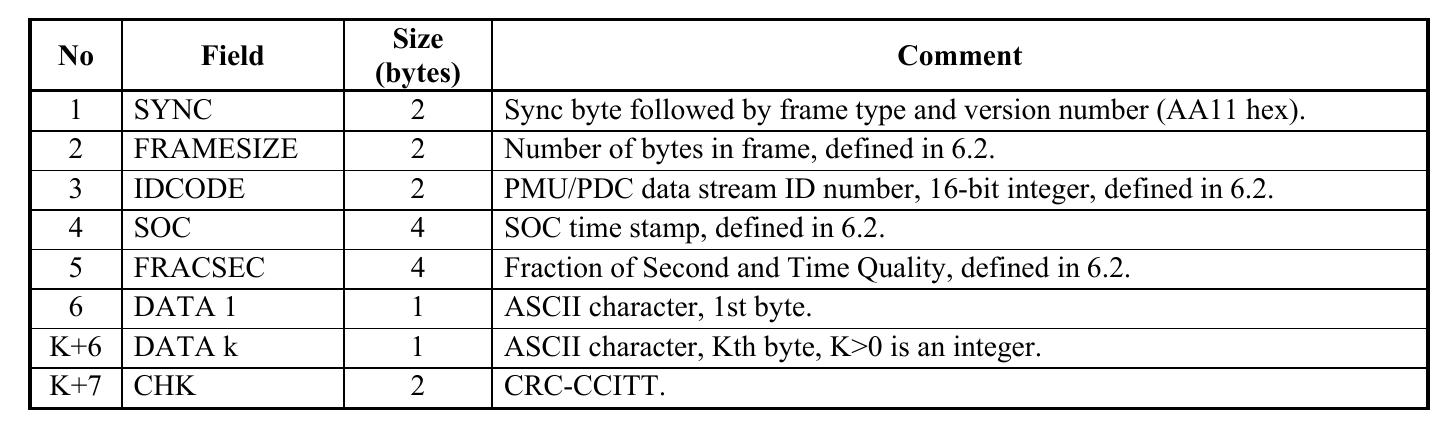
\includegraphics[width=\textwidth]{fig/hdr_frame.png}
	\caption{Header Frame structure \cite{c37.118.2}}
\end{figure}

\begin{figure}[h]
	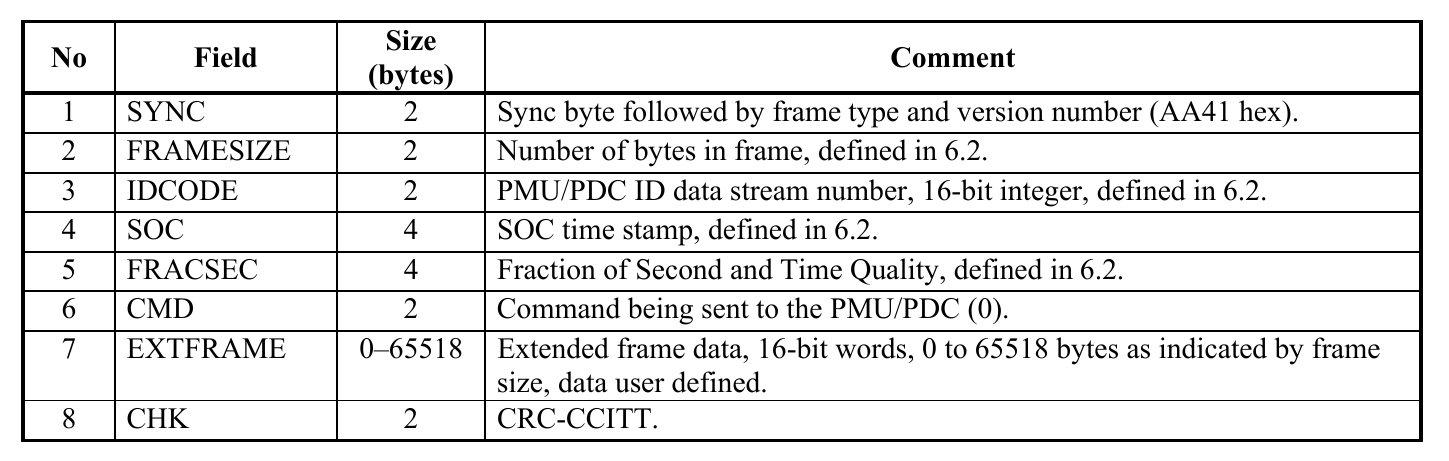
\includegraphics[width=\textwidth]{fig/cmd_frame.png}
	\caption{Command Frame structure \cite{c37.118.2}}
\end{figure}

\begin{figure}[h]
	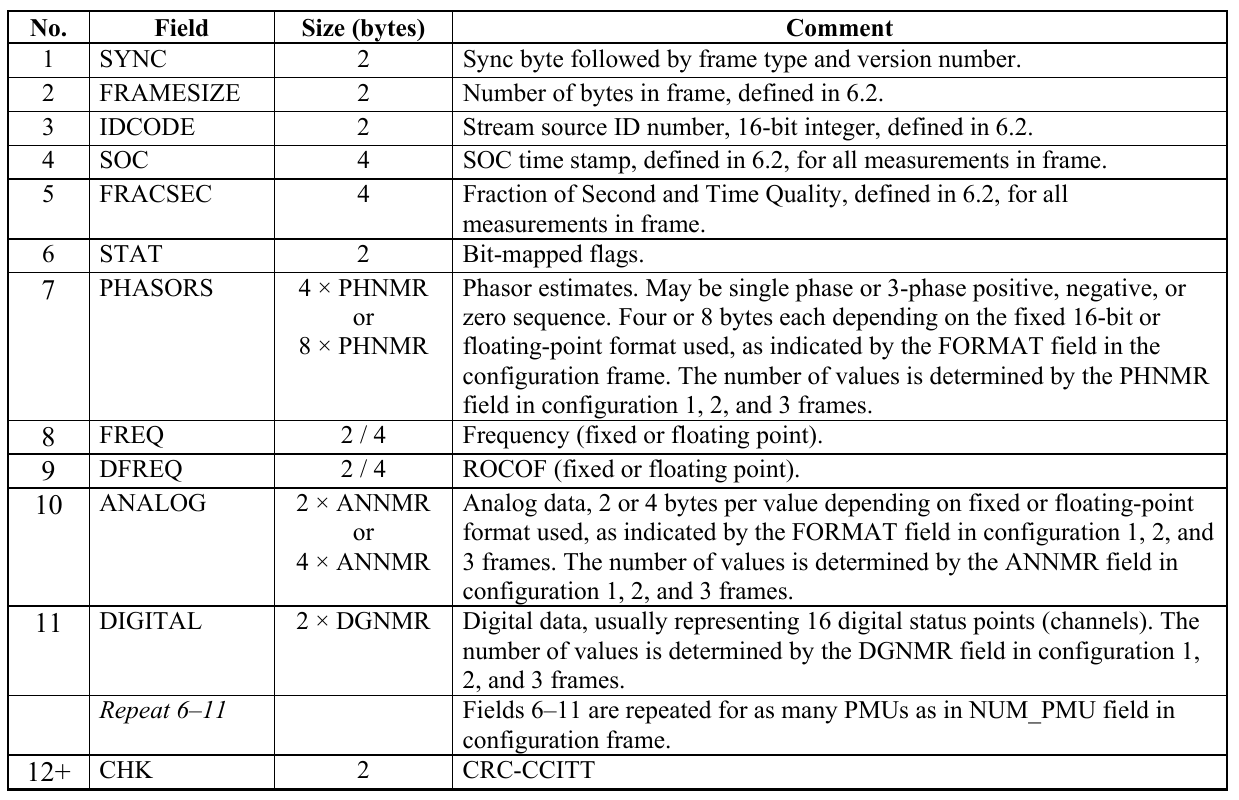
\includegraphics[width=\textwidth]{fig/data_frame.png}
	\caption{Data Frame Structure \cite{c37.118.2} }
\end{figure} 


\begin{figure}[h]
	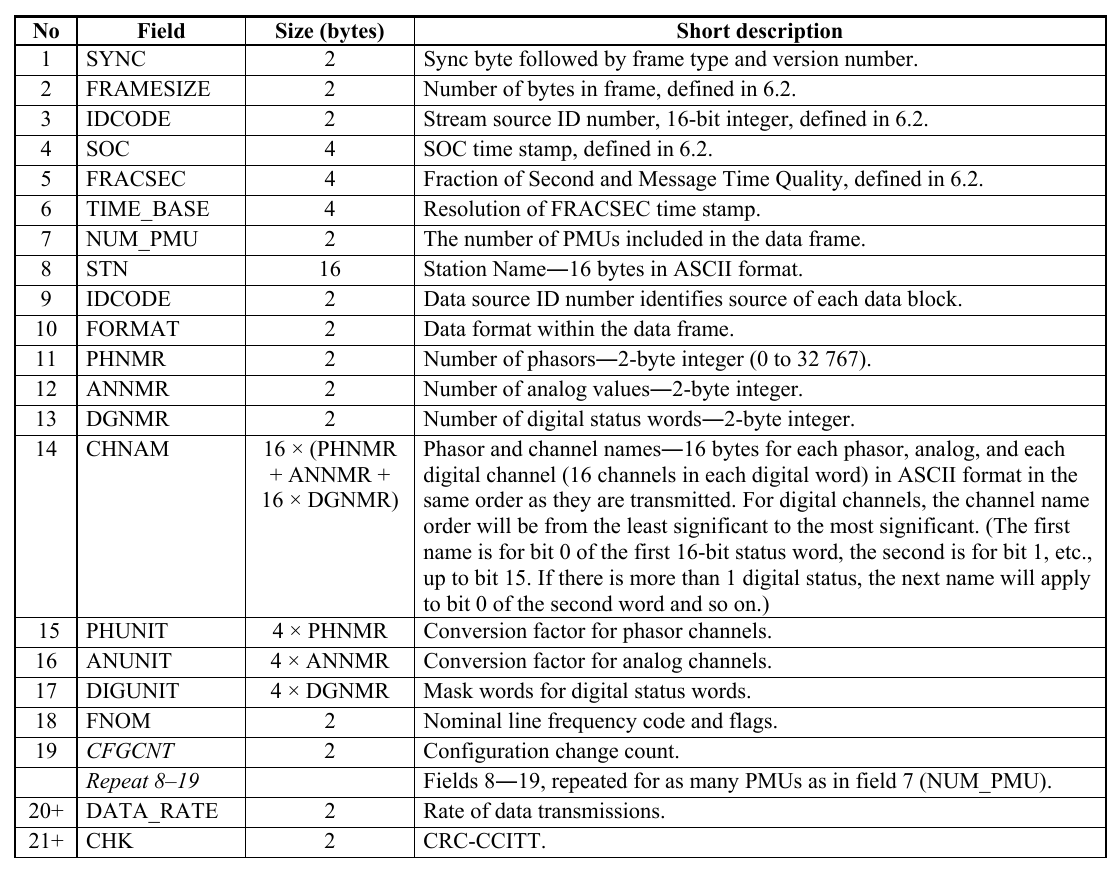
\includegraphics[width=\textwidth]{fig/cfg_frame12.png}
	\caption{Configuration Frame 1 - 2 Structure \cite{c37.118.2}}
	\label{fig:cfg_12}
\end{figure} 

Following configurations shown in Fig:\ref{fig:cfg_12} and in Fig: \ref{fig:cfg_3} are machine readable messages communicated before the data frame is sent. They are the full description of device status and capability, here only brief details are given, further details can be read from the standards- C37.118.2   
\begin{figure}[h]
	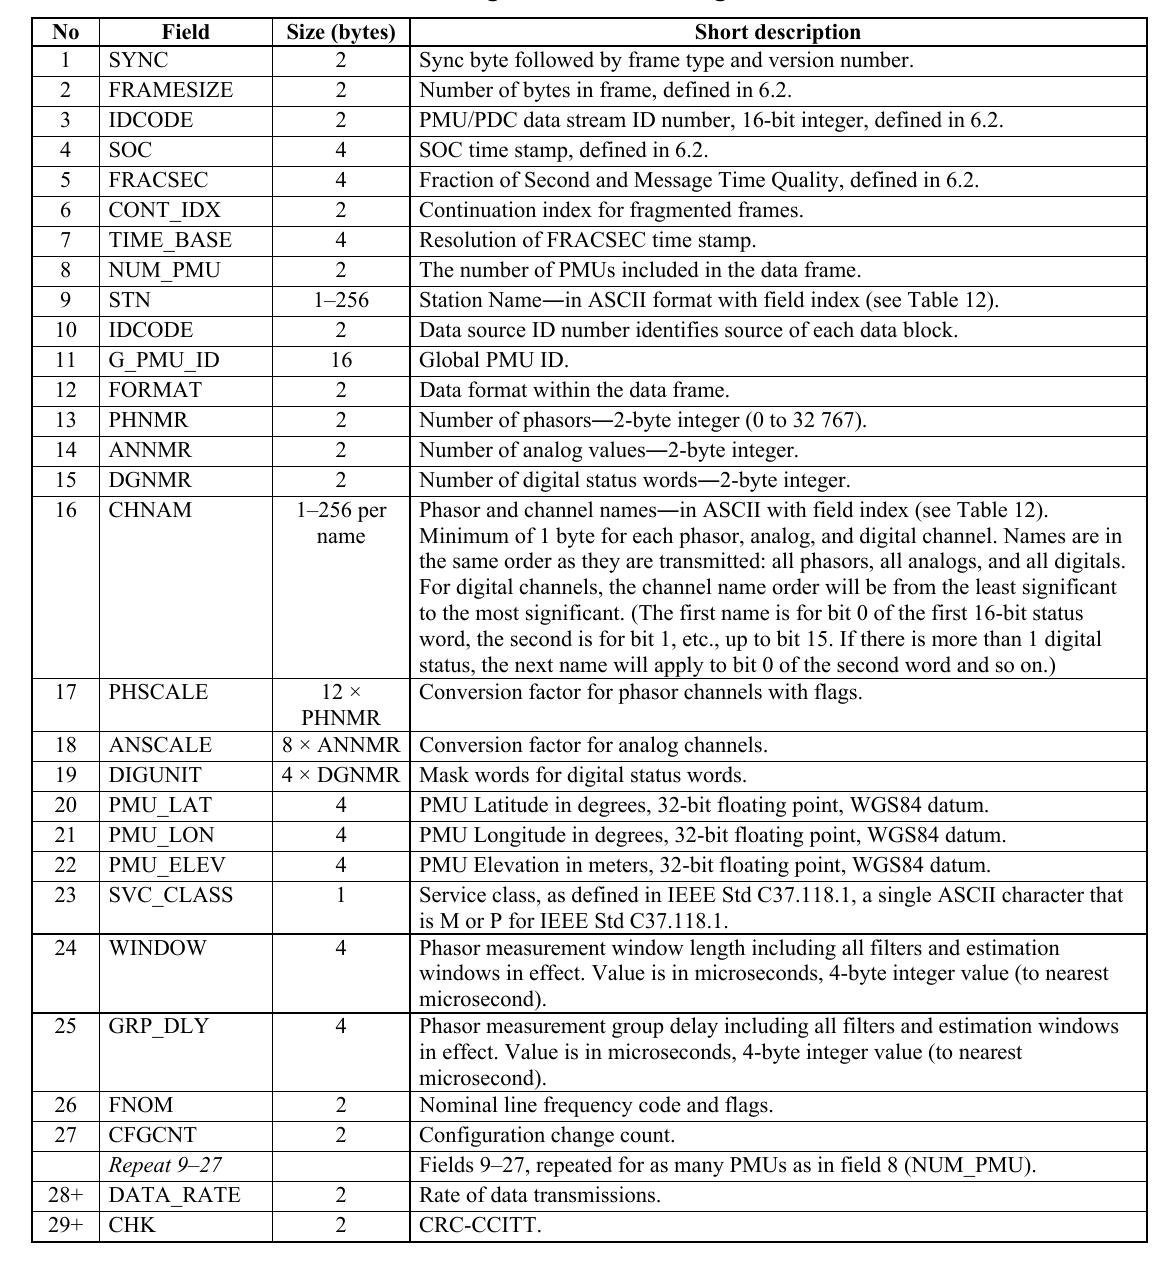
\includegraphics[width=\textwidth]{fig/cfg_frame3.png}
	\caption{Configuration Frame 3 Structure \cite{c37.118.2}}
	\label{fig:cfg_3}
\end{figure} 


\end{appendix}
